\centerline{\bf I. Introduction}
\addcontentsline{toc}{subsection}{I. Introduction}
\smallskip


The discovery of an inhabited planet is a primary goal of exoplanetary
science. The \kepler~spacecraft has now found several small candidates
in potentially habitable orbits, \cite[e.g. Kepler--62
  f;][]{2013arXiv1304.7387B}, and radial velocity surveys are also detecting
apparently low--mass planets in habitable zones (HZs), e.g. Gl 667C c
\citep{AngladaEscude12}.  While the location of an orbit with respect
to the HZ is an important first cut, the composition of the planet is
at least as important.  Life as we understand it cannot survive on
gaseous planets, yet we do not know the mass and/or radius that
separates gaseous from terrestrial planets.  In particular, the
identification of the critical radius between the two, $R_{crit}$,
would provide crucial information for \kepler's primary mission to
discover a terrestrial planet in the HZ of a G dwarf.

The primary goal of this proposal is to determine this critical
planetary radius between rocky and gaseous bodies using \kepler~data.
We will exploit the expected discrepancy in tidal dissipation of
gaseous and rocky bodies to determine the largest orbital periods at
which the two classes of bodies circularize.  We will use the
so--called transit duration deviation, the difference between the
observed transit duration and that of a circular orbit, to estimate
the minimum eccentricity permitted from the transit data.  We will
also include the effects of additional planetary companions and
atmospheric mass loss, as they also influence the evolution of
eccentricity.  In order to successfully constrain these theoretical
results from \kepler~data, we require robust characterization of each
candidate, and hence we will perform state--of--the--art transit
modeling of all relevant \kepler~transits.  To optimize our
sensitivity to these effects, we will examine only those systems with
short periods (less than 10 days) and having planetary radii near the
anticipated boundary (less than 4 \rearth).  Our proposed research
offers the best route to determine which \kepler~candidates are rocky,
independent of mass measurements, which is vital information in
\kepler's quest to discover potentially habitable planets orbiting G
dwarfs.  In summary:

\par\smallskip\noindent
\centerline{
  \begin{minipage}[c]{0.9\textwidth}
    {\bf We propose to exploit the observed minimum eccentricity, tidal
      theory, and a reanalysis of \kepler~data to determine $R_{crit}$, as
      well as constrain the tidal quality factors of both rocky and
      gaseous planets ($Q_r$ and $Q_g$, respectively), and the efficiency
      of hydrogen loss for close in small gaseous exoplanets in the
      \kepler~field.}
  \end{minipage}
}
\par\smallskip\noindent

\bigskip
\centerline{\bf II. Objectives and Significance}
\addcontentsline{toc}{subsection}{II. Objectives and Significance}
\smallskip

\medskip
{\centerline{\ub{\sc Tidal Theory}}}
\smallskip

Tidal dissipation is celestial bodies in extremely challenging to
measure
\citep{GoldreichSoter66,Hut81,AksnesFranklin01,Jackson08a,Jackson09,Lainey12}
due to 1) the dearth of worlds in highly dissipative configurations,
2) the long timescales involved (Gyrs), and 3) the intractability of
derivations based on first principles.  However, the \kepler~ space
telescope has now discovered thousands of exoplanet candidates
\citep{2013ApJS..204...24B}, of which about 1000 orbit FGK stars with
orbital periods less than 10 days, and that may experience significant
tidal evolution \cite{Rasio96,Jackson08a,Matsumura10}.

In the equilibrium tide model
\citep{Darwin1880,MacDonald64,GoldreichSoter66,Hut81,FerrazMello08,Leconte10},
the figure of a tidally deformed body is a superposition of surface
waves with different frequencies.  The sum of these waves corresponds
to the tidally--deformed figure, and allows for the relatively simple
derivation of the time rates of change of orbital and spin properties.
While two qualitatively different models have emerged, the
constant--phase--lag (CPL) and constant--time--lag (CTL) models
\citep{Greenberg09}, both rely on this assumption of superposition,
and neither has been rejected observationally.  Both models make a
critical prediction that we will exploit in this proposal: The tidal
dissipation in rocky planets is orders of magnitude larger than in
gaseous bodies.  This disparity implies that rocky planets will evolve
much more rapidly than gaseous bodies and we expect rocky exoplanets
to be tidally circularized on larger orbits than for gaseous bodies.
As we show below, the canonical values for $Q_g$ of $10^6$ and $Q_r$
of 100 should be measurable in the \kepler~field, if the transit data
and stellar properties can be known to sufficient accuracy.  The key
is to recognize that gaseous bodies will tidally circularize more
slowly than rocky planets, and may still retain non--zero
eccentricities after Gyrs.  While transit data cannot measure the
eccentricity \citep{Barnes07}, they {\it can} provide a lower limit,
which we outline below.

\medskip
{\centerline{\ub{\sc The Transit Duration Deviation (TDD)}}}
\smallskip

The transit duration is the time required for a planet to traverse the
disk of its parent star, and to first order is:
\begin{equation}\label{eq:duration}
T = \frac{\sqrt{R_*^2 - b^2}}{v},
\end{equation}
where $R_*$ is the radius of the star, $b$ is the impact parameter,
and $v$ is the instantaneous velocity of the planet. On a circular
orbit, $v$ is constant and we expect
\begin{equation}\label{eq:durcirc}
T_c = \frac{\sqrt{R_*^2 - b^2}}{\pi a}P,
\end{equation}
where $P$ is the orbital period. However, for an eccentric orbit the
orbital velocity is a function of longitude (Kepler's 3rd Law), and is
given by
\begin{equation}\label{eq:velocity}
v(\theta) = \frac{2\pi a}{P}\sqrt{\frac{1 + 2e\cos(\theta) + e^2}{1-e^2}},
\end{equation}
where $e$ is the eccentricity and $\theta$ is the true anomaly, the
angle between the longitude of pericenter and the actual position of
the planet in its orbit. From transit data alone, the value of
$\theta$ is unknown, and hence so is $e$.

However, we can exploit the difference between $T$ and $T_c$ to obtain
a minimum value of the eccentricity, $e_{min}$ \citep{Barnes07}. The
situation is somewhat complicated because $T$ can be larger or smaller
than $T_c$ depending on $\theta$. If the planet is close to apoapse,
$T > T_c$, while at periapse $T < T_c$. To derive $e_{min}$ we must
assume that $\theta = 0$ or $\pi$. While the velocity could be larger
at some other position in the orbit, we know that the maximum
deviation from the circular velocity is at least as large as the
measured velocity, and hence $e$ must be at least a certain value. If
we define the transit duration deviation, $\Delta$, as
\begin{equation}\label{eq:tdd}
\Delta = \begin{dcases} \frac{T-T_c}{T_c} & T_c < T \\ \frac{T_c - T}{T_c} & T_c > T, \end{dcases}
\end{equation}
and then for ease of notation,
\begin{equation}\label{eq:deltaprime}
\Delta' \equiv \begin{cases} \Delta + 1 & T_c < T \\ \Delta - 1 & T_c > T, \end{cases}
\end{equation}
then we find that
\begin{equation}\label{eq:emin}
e_{min} = \begin{dcases} \frac{\Delta'^2 - 1}{\Delta'^2 + 1} & T_c < T \\ \frac{1 - \Delta'^2}{1 + \Delta'^2} & T_c > T \end{dcases}
\end{equation}
is the minimum eccentricity permitted by transit data.  We use the
absolute value of $e_{min}$ in our discussions below.

\medskip
{\centerline{\ub{\sc The Boundary Between Rocky and Gaseous Planets}}}
\smallskip

That transit data provide a minimum eccentricity while tidal theory
damps eccentricity to zero is crucial for our proposed research. If
$e_{min} = 0$, \textit{then the orbit is circular}.  Of course circular
orbits could be primordial, but \cite{Jackson08,Matsumura10} showed
that the observed radial--velocity--detected planets in tight orbits
could have formed with eccentricities consistent with the more distant
planets and were subsequently tidally damped in both the CPL and CTL
framework.  If $e_{min} > 0$ then tides have not tidally damped the
eccentricity, and, if we know the age of the system, then we can
estimate the tidal $Q$ (or in the CTL model, the time lag factor).

As an example consider the two curves in Fig.~\ref{fig:compareQ}.
Both these planets begin with the same orbit around the same star.
The line shows 10 Gyr of tidal evolution of a 2~\rearth planet with a
density of 1 g/cm$^3$ and tidal $Q$ of $10^6$ (i.e. a 3.8~\mearth
``mini-Neptune''), while the filled circles represent the orbit of a
2~\rearth planet with a mass of 10~\mearth and a tidal $Q$ of 100
(i.e. a ``super-Earth'') every 100 Myr.  The super--Earth circularizes
in about 1 Gyr; the mini--Neptune does not evolve significantly, even
after 10 Gyr.  This discrepancy is evident despite the fact that
equilibrium tidal models predict that evolution scales as mass to the
3/2 power and radius to the fifth power -- instead, the large
difference between the $Q$s dominates.  We therefore hypothesize that
the TDD may be able to identify the radius that separates gaseous
planets from rocky planets.

\begin{figure}[h]
\centering
\begin{minipage}{2.7in}
\resizebox{2.7in}{!}{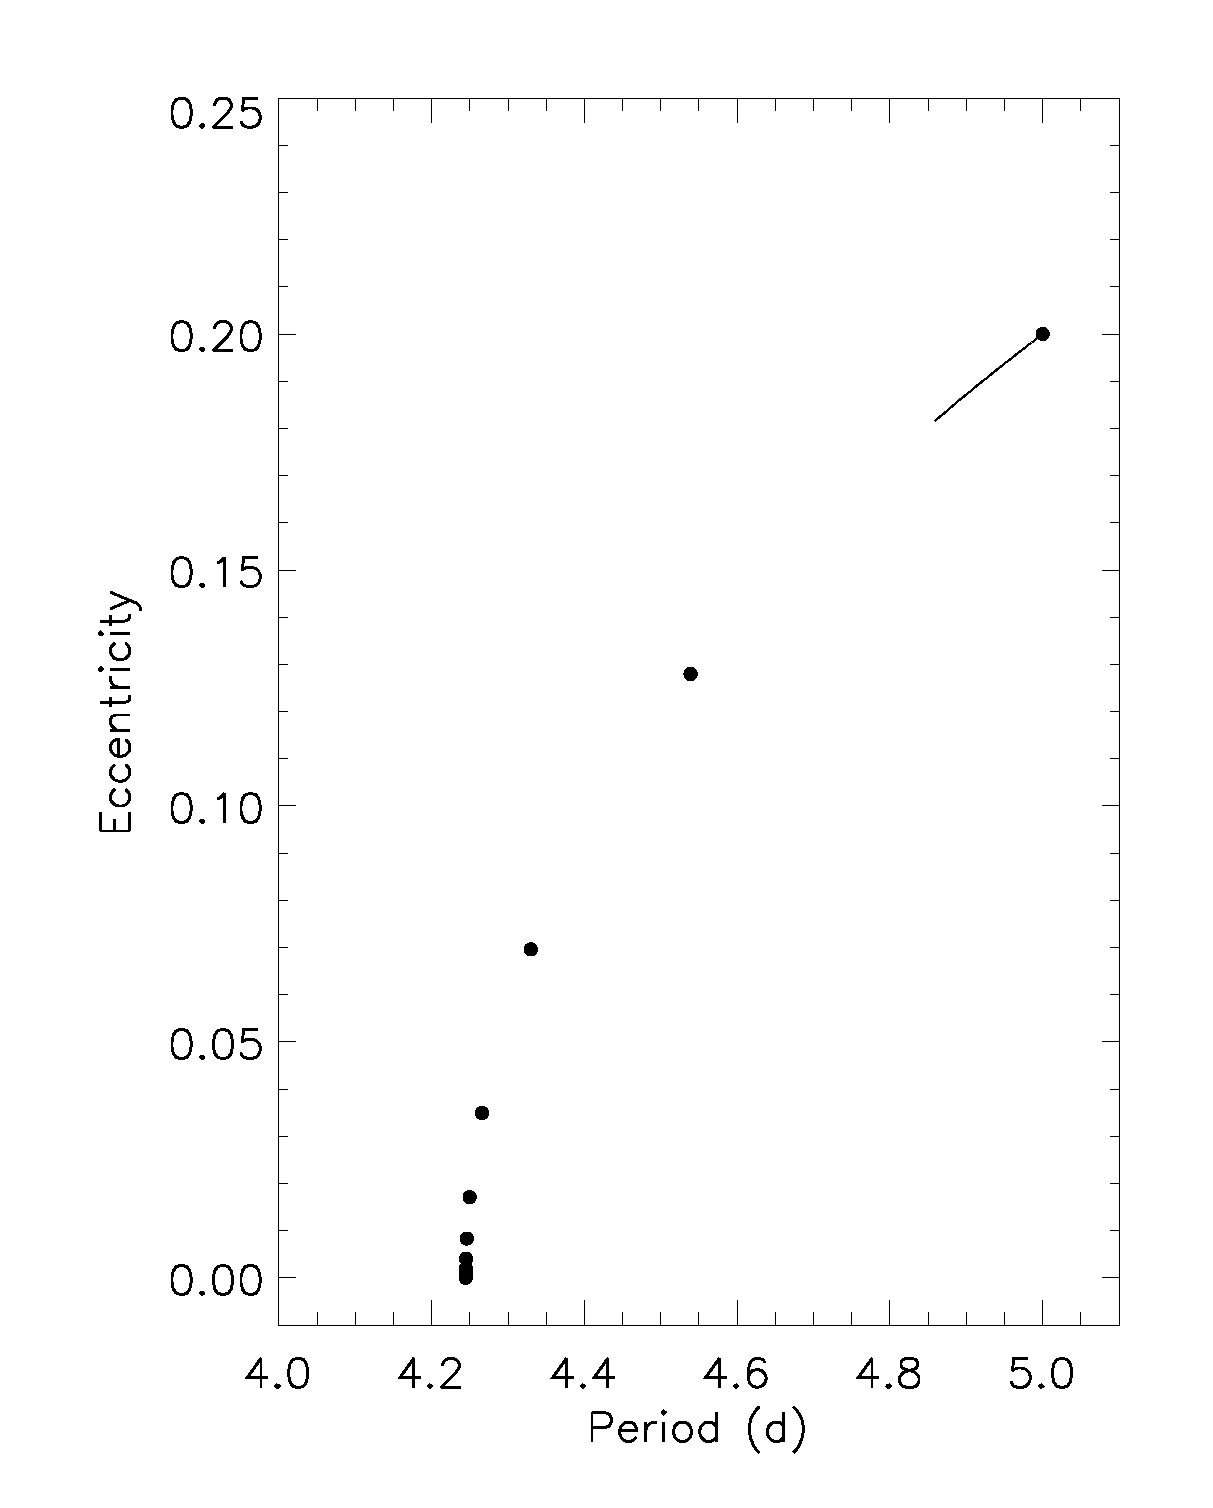
\includegraphics{figures/compq.ps}} 
\end{minipage}
\begin{minipage}{2.7in}
\caption{\label{fig:compareQ}Comparison of the tidal evolution of a
  2~\rearth mini--Neptune (solid line; for 10 Gyr) and a 2~\rearth
  super--Earth (circles; in 100 Myr intervals).  The mini--Neptune
  experiences little orbital evolution, but the super--Earth
  circularizes in about 1 Gyr.  This discrepancy is due to the 4
  orders of magnitude difference in tidal dissipation between gaseous
  and rocky planets.}
\end{minipage}
\end{figure}

To test this possibility, we performed the following test. We created
25,000 synthetic star--planet configurations with initial semi--major
axes uniformly in the range [0.01,0.1] AU, radii in the range
[0.5,10]~\rearth, stellar masses in the range [0.8,1.2]~\msun, and
ages in the range [2,8] Gyr.  If the radius is less than 2~\rearth, we
scale the mass as ($R$/\rearth)$^{3.68}$\mearth \citep{Sotin07} and we
assign a tidal $Q$ in the range [30,300].  If larger, then we assume
the density is 1 g/cm$^3$, and a tidal $Q$ in the range
[$10^6$,$10^7$].  The initial eccentricity is drawn from the currently
observed distribution of distant planets ($a > 0.2$~AU).  We then
integrate the system forward for the randomly chosen age and assume we
observe the system in that final configuration. In Fig.~\ref{fig:radper},
we show the resulting average eccentricities of these planes as a
function of planetary radius, $R_p$, and orbital period, $P$.  The
small values of $e$ at low $R_p$ and $P$ shows this effect.
Furthermore, we can see the features that correspond directly to three
parameters that are currently very poorly constrained: $R_{crit}$ via
the rapid rise in $\avg{e}$ at 2~\rearth; $Q_g$ via the rapid rise in
$\avg{e}$ at 1 day above 2~\rearth; and $Q_r$ via the rapid rise at 4
days and below 2~\rearth.  Thus in this simple model, we see three
constraints for three unknowns, yielding the possibility that the
right observations may be able to provide values to these elusive
quantities.

\begin{figure}[h]
\centering
\begin{minipage}{2.7in}
\resizebox{2.7in}{!}{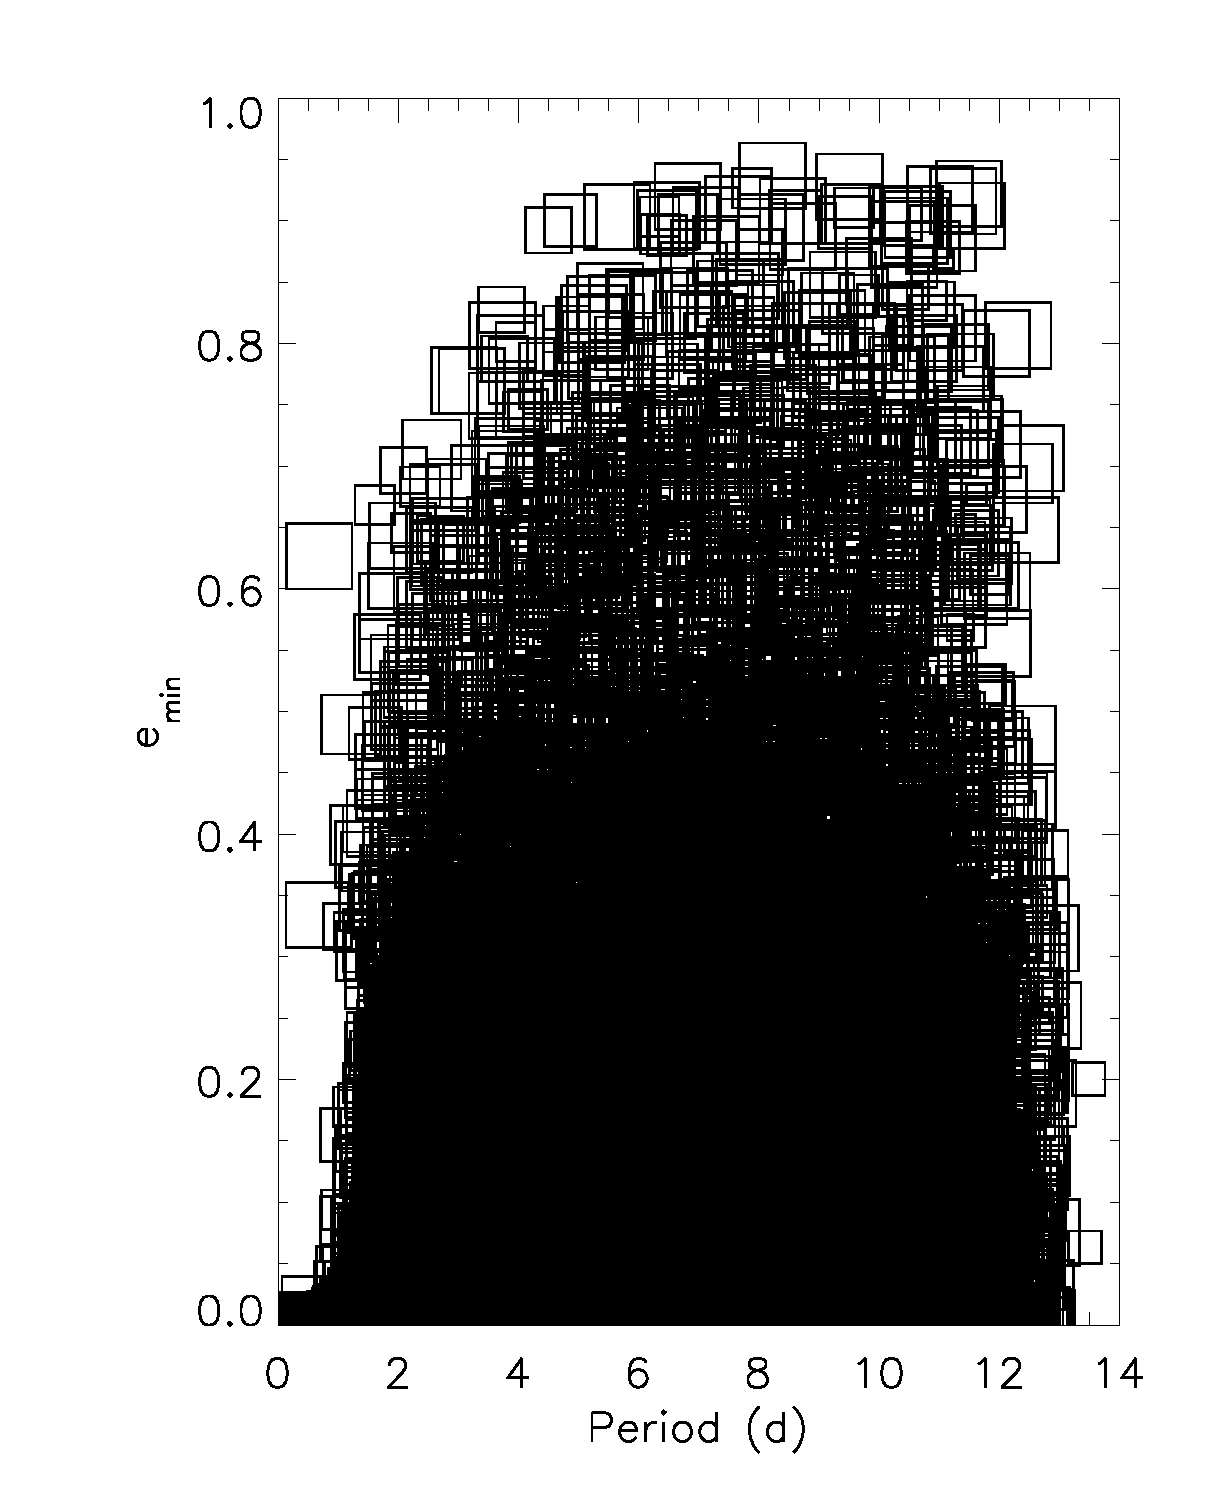
\includegraphics{figures/radper.ps}} 
\end{minipage}
\begin{minipage}{2.7in}
\caption{\label{fig:radper}Average final eccentricity of a suite of 25,000
systems of one star and one planet. Planets larger than 2~\rearth~are gaseous, and 
those smaller are rocky. The binsizes are 0.5~\rearth in radius and 0.5 d in period.
Gaseous planets retain a residual eccentricity if $P > 1.5$ d, while rocky planets require
$P > 4$ d. The transition occurs at 2~\rearth, which in this case is $R_{crit}$. }
\end{minipage}
\end{figure}


However, \kepler~data do not provide eccentricity, but rather the
minimum eccentricity. We must therefore transform these data into a
form that is directly comparable to an observable, e.g. $e_{min}$. In
order to calculate $e_{min}$, we choose a random value for $\theta$
and calculate the velocity according to Eq.~\ref{eq:velocity}. We
calculate the average minimum eccentricity, $\avg{e_{min}}$ in
1~\rearth~planetary radius bins and 1 day orbital period bins and plot
$\avg{e_{min}}$ as a function of orbital period for different radii as
solid lines in Fig.~\ref{fig:emin}. For $R < 2$~\rearth, $\avg{e_{min}}
\sim 0$ up to about a 4 day period. However, for larger radii,
circular orbits are only guaranteed for periods less than about 2
days. \textit{Despite the order of magnitude ranges for each physical
  planetary property, the disparity in tidal $Q$'s produces a strong
  signal in $\avg{e_{min}}$ that distinguishes the rocky and gaseous
  planets. }

\begin{figure}[h]
\centering
\begin{minipage}{2.7in}
\resizebox{2.7in}{!}{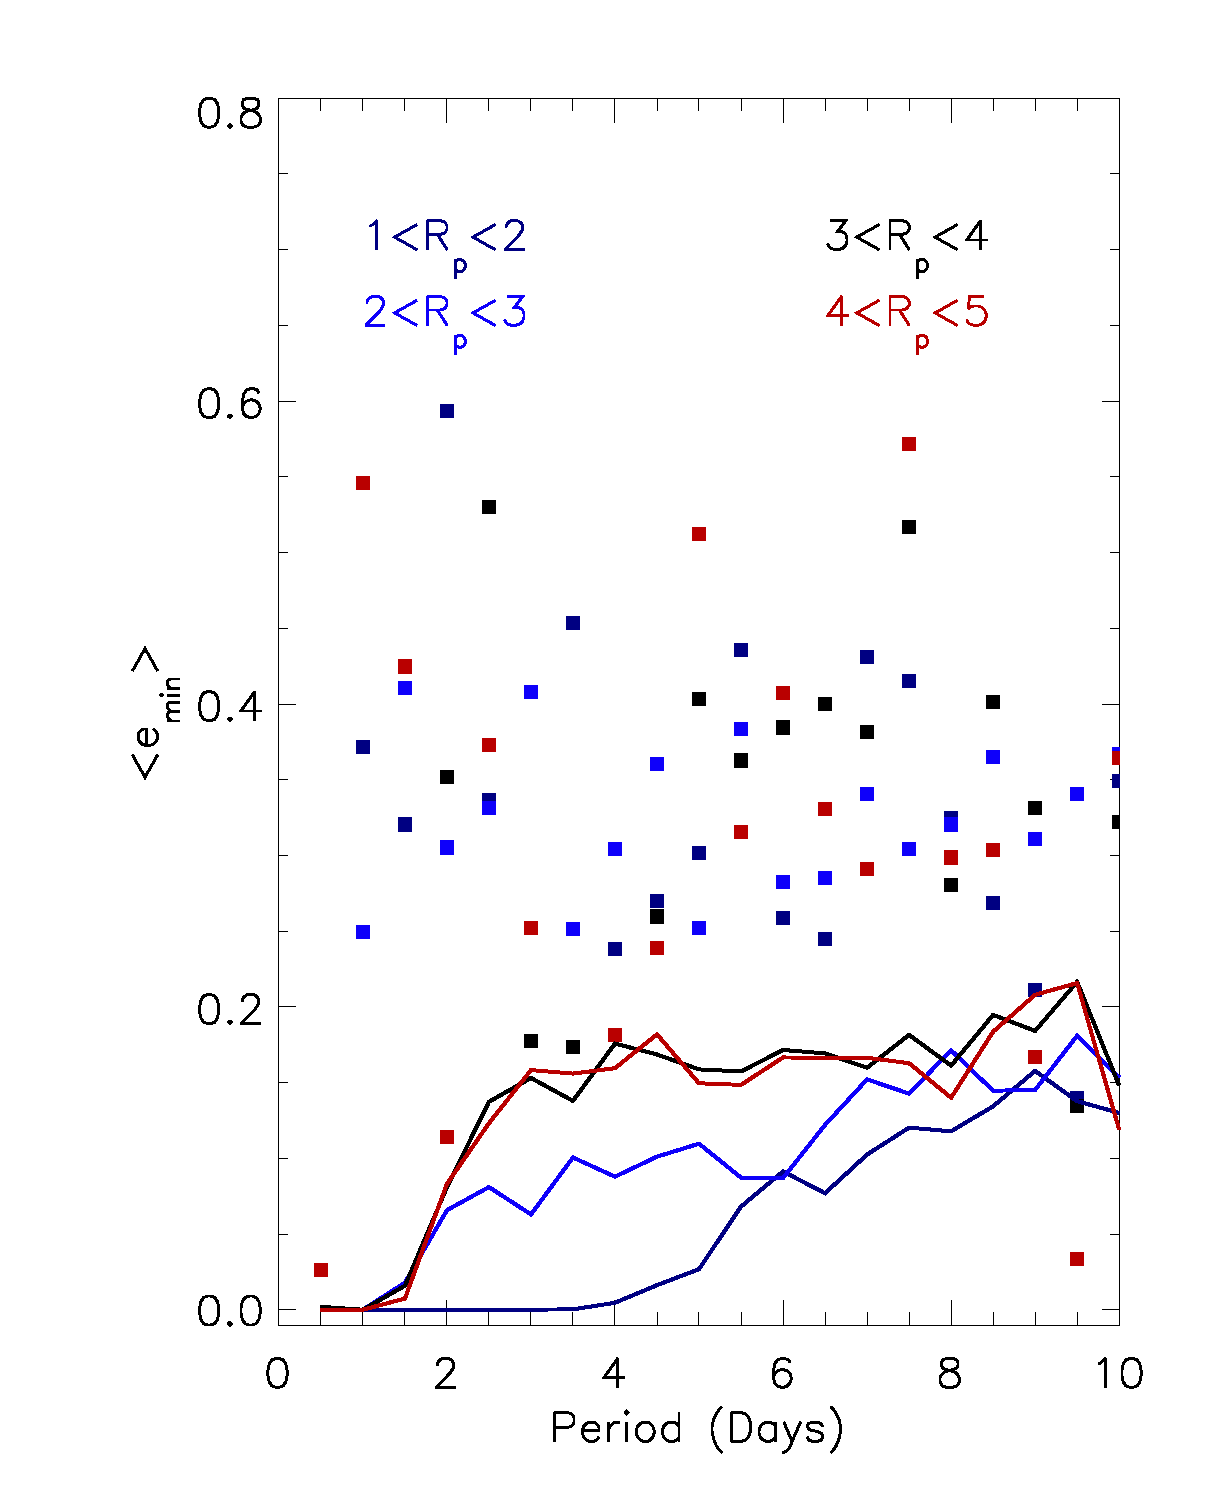
\includegraphics{figures/compare.emin.ps}} 
\end{minipage}
\begin{minipage}{2.7in}
\caption{\label{fig:emin}Average minimum eccentricities for transiting
  exoplanets as a function of period and radius.  Solid curves
  correspond to a theoretical study of 25,000 star--planet
  configurations in which planets with $R < 2$\rearth are rocky and
  larger planets are gaseous.  Note that gaseous planets have
  non--zero eccentricities if the period is larger than 1.5 days,
  whereas rocky planet periods must be larger than 4 days.  Filled
  squares are the values for observed \kepler~planets as provided by
  JPL's \kepler~website.  The observed systems appear to be not
  well--characterized, and hence a proper re--analysis of the
  \kepler~planets is required to identify the radius that separates
  rocky and gaseous planets, as well as both values of tidal $Q$.}
\end{minipage}
\end{figure}

This pilot study is encouraging, but its feasibility rests on the
precision of the models of the \kepler~data.  Specifically, impact
parameters, stellar and planetary radii, orbital period, and stellar
mass must be known and their uncertainties well--modeled.  The first
four properties are measurable from transit data alone, while the
fifth must be estimated by other means.  The \kepler~team has provided
these data in various publications and websites.  The solid squares
show the values of $\avg{e_{min}}$ with quantities from the
\kepler~Planet Candidate Data
Explorer\footnote{http://planetquest.jpl.nasa.gov/kepler}.  All the
observed data are above the predictions. There are two possible
explanations for this discrepancy: 1) The theory is wrong, or 2) the
reported model parameters are of poor quality.  We outline limits of
the theory below.

\medskip
{\centerline{\ub{\sc Non--Tidal Effects}}}
\smallskip

First, we note that additional companions can pump eccentricity
through mutual gravitational interactions, even if tidal damping is
ongoing \citep{MardlingLin02,Bolmont13}.  Therefore we must
be cautious when interpreting Fig.~\ref{fig:pilot}, as additional
companions, both seen and unseen, can maintain non--zero
eccentricities.  However, \cite{Bolmont13} showed that planet--planet
interactions cannot maintain 55 Cnc e's eccentricity above 0.1.  That
system is particularly relevant as there are many close--in planets
orbiting G dwarfs.  Therefore, we can conclude that discrepancy
between the observed and simulated systems is not due to
planet--planet interactions.

Another possibility is that stellar winds and activity can strip an
atmosphere, reducing the mass and radius, and potentially changing the
planet from a mini--Neptune to a super--Earth
\citep{Jackson10,Valencia10,Leitzinger11,Poppenhaeger12}.  Recently,
\cite{OwenWu13} argued that the \kepler~sample is consistent with
hydrodyanmic mass loss, and that some low--mass planets could have
formed with substantially more mass.  Mass loss should decrease the
time to circularize the orbit, assuming the radius doesn't become very
large, which is unlikely after about 100 Myr \citep{Lopez12}.
Therefore, mass loss could stall circularization for mini--Neptunes,
but not for super--Earths.  Although few radial velocity measurements
exist, planets with radii less than $\sim 1.5$~\rearth~ have densities
consistent with silicate compositions \citep{Batalha10}.  Thus, mass
loss seems unlikely to explain the discrepancy seen for the smallest
candidates in the \kepler~field.

Other effects, such as stellar mass loss or the galactic tide will be
negligible, but to properly treat the problem, planetary mass loss and
planet--planet perturbations must be considered.  On the theoretical
side, the path forward to determine $R_{crit}$, $Q_{r}$ and $Q_{g}$ is
clear: We must first model the full range of plausible values for
these three parameters to calculate $\avg{e_{min}}$($R_p,P$).  We must
then include the planet--planet interactions of multiple planet
systems over the lifetimes of the systems.  Finally, we must
incorporate mass loss, including the possibility that a mini--Neptune
can become a super--Earth with its associated change in tidal $Q$.

\bigskip
\centerline{\bf III. Technical Approach and Methodology}
\addcontentsline{toc}{subsection}{III. Technical Approach and Methodology}
\smallskip

%\medskip
%{\centerline{\ub{\sc Transit Duration}}}
%\smallskip
%
%What is this definition?  Center of planet crossing?
%
%\begin{eqnarray}
%\Delta t_{circ} & = & {{P}\over{\pi}}~{{\sqrt{R_*^2 - b_0^2}}\over{a}} \nonumber \\
%                & = & {{P}\over{\pi}}~{{\sqrt{1 - \beta_0^2}}\over{\alpha}}
%\label{eq-tcirc}
%\end{eqnarray}
%where $P$ is the orbital period in cgs units, $R_*$ the stellar radius
%in cgs, $b_0$ the minimum planetary impact parameter in cgs, $\beta_0$
%a unitless measure of the minimum impact parameter (scaled by the
%stellar radius), $a$ the planetary semi--major axis in cgs, and
%$\alpha$ this value scaled by the stellar radius.


\medskip
{\centerline{\ub{\sc Transit Model}}}
\smallskip

To avoid a dependency between the fitted model and a physical model
that includes orbital dynamics, we parameterize the fitted lightcurve
in purely geometric terms.  To do so, we adopt the quadratic
limb--darkened model of \cite{2002ApJ...580L.171M}, which describes
transit lightcurves in terms of two (nuisance) limb--darkening
coefficients and two (important) system parameters.  The first of the
system parameters is the planetary radius divided by the stellar
radius ($\zeta \equiv Rp/R_*$), which determines the fractional area
of the stellar disk that may be occulted by the planet.  The second is
the impact parameter of the planet ($\beta \equiv b/R_*$).  This
variable is a function of time due to the objects' relative motion.
This function is dependent on the chord that the planet takes across
the stellar disk, itself typically estimated using the orbital
parameters semi--major axis ($\alpha \equiv a/R_*$) and inclination.

Instead we use here a purely geometric parameterization, represented
in Figure~\ref{fig-schem}.  We describe the impact parameter as a
function of time using the minimum impact parameter $\beta_0$ -- when
the centers of the sources are aligned along the x--axis at
center--of--transit time $t_0$ -- and the location of the planet on
the transit chord across the stellar disk.  The x--coordinate of the
planet as a function of time is represented as $x(t) / R_* = (t - t_0)
* v_\perp / R_* = (t - t_0) / \tau$, where $v_\perp$ is the (unknown)
perpendicular velocity, and $\tau$ is the (fitted) amount of time it
takes the planet to traverse a distance equal to the stellar radius
assuming no acceleration.  This allows us to express geometrically the
impact parameter as a function of time:
\begin{eqnarray}
\beta(t) & = & \sqrt{\beta_0^2 + \left((t - t_0) / \tau\right)^2},
\end{eqnarray}
which is then used along with $\zeta$ to generate a model transit
lightcurve.
This model yields a 4--parameter fit to each transit: $t_0, \beta_0^2,
\tau, \zeta$.  The system period $P$ may be determined using the
ensemble of $t_{0;i=1...N}$.
The transit duration $T$ may be found from the 2 solutions to
$\beta(t) = 1$, and represents the time between the center of the
planet crossing each limb of the star:
\begin{eqnarray}
T & = & 2 * \tau \sqrt{1 - \beta_0^2}.
\label{eq-dt}
\end{eqnarray}

Combining Equations~\ref{eq:tdd}--\ref{eq:emin} with
Equation~\ref{eq-dt}, we express $e_{min}$ in terms of our model
parameters:
\begin{eqnarray}
e_{min} & = & \pm \frac{P^{2} - 4 \pi^{2} \alpha^{2} \tau^{2}}{P^{2} + 4 \pi^{2} \alpha^{2} \tau^{2}}
\label{eq-emin2}
\end{eqnarray}
All factors of the minimum impact parameter $\beta_0$ cancel out,
which is fortuitous as this is typically the least constrained of all
system parameters, especially for the long--cadence \kepler data.
While the uncertainty in $\beta_0$ will affect our knowledge of the
other system parameters, this uncertainty may be marginalized over by
examining the posterior distributions, which drives us to use
Markov--Chain Monte Carlo (MCMC) modeling (described below).

Equation~\ref{eq-emin2} indicates that $e_{min}$ is purely a function
of the fitted parameter $\tau$, the derived period $P$, and an assumed
semi--major axis for the planet (in units of the stellar radius)
$\alpha$.  The uncertainty in $e_{min}$ scales as below for all 3
parameters:

\begin{eqnarray}
\Xi & \equiv & \frac{16 \pi^{2} \alpha^{2} \tau^{2} P^{2}}{16 \pi^{4} \alpha^{4} \tau^{4} - P^{4}} \\
\frac{\delta e_{min}}{\delta \xi} & = & \frac{\Xi~e_{min}}{\xi} ~~~~~ \left[\xi = \tau; P; \alpha \right].\nonumber
\label{eq-emin3}
\end{eqnarray}
In the limit of a circular orbit ($P \rightarrow 2 \pi \alpha \tau$),
$\Xi~e_{min}$ = 1.

\begin{figure*}[t] 
  \begin{minipage}[c]{0.37\textwidth}
    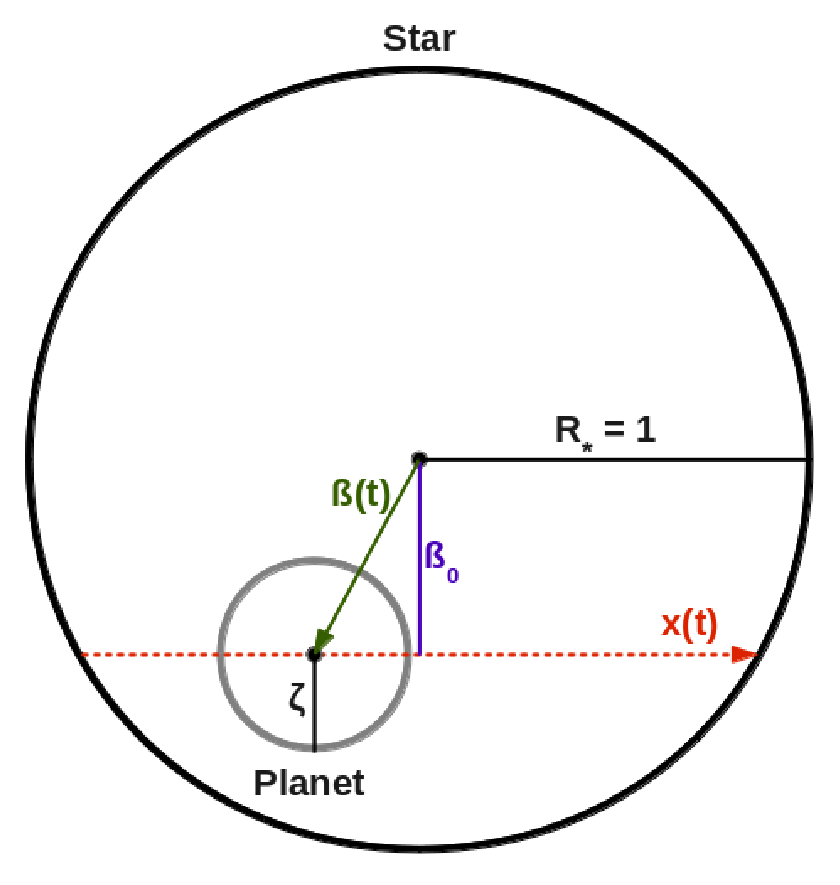
\includegraphics[width=\textwidth]{figures/schem.eps}
  \end{minipage}\hfill
  \begin{minipage}[c]{0.6\textwidth}
    \caption{Schematic detailing our geometric model for the impact
      parameter as a function of time, $\beta(t)$.  Relevant variables
      include the minimum impact parameter scaled by the stellar radius
      $\beta_0$, the radius of the planet scaled by the stellar radius
      $\zeta$, and the time-dependent position of the planet $x(t)$.  The
      fitted parameters are $t_0$ (defined where $\beta(t_0) = \beta_0$),
      the minimum impact parameter $\beta_0$, scaled planetary radius
      $\zeta$, and $\tau$ (which represents the time for the planet to
      travel the angular distance subtended by the stellar radius). }
    \label{fig-schem}
    \hspace*{\fill}  
    \hrule
  \end{minipage}
\end{figure*}

%\medskip
%{\centerline{\ub{\sc Simulations}}}
%\smallskip
%
%We use the system inclination, semi--major axis, planet--to--star
%radius ratio, and period (along with two limb darkening parameters) to
%generate fake system lightcurves using the method of
%\cite{2002ApJ...580L.171M}.  The system lightcurve is evaluated once
%each minute and integrated over 30 evaluations to approximate a single
%\kepler long--cadence observation.  This is done for a window of 1 day
%on either side of the given transit midpoint to ensure significant
%out--of--transit data to include in the fit.  We perform these
%evaluations for all transits for 14 ``quarters'' of \kepler
%observations, or approximately 1280 days.
%
%A white--noise component is added to each lightcurve for each of 4
%magnitude bins, using the precisions in parts--per--million (ppm)
%given on the \kepler calibration
%webpage \footnote{http://keplergo.arc.nasa.gov/CalibrationSN.shtml}.
%We evaluate each lightcurve separately for magnitude 8/10/12/14
%objects, adding a random contribution of amplitude 11.3/29/80/296 ppm
%(respectively) to each datapoint as generated above.  We do not
%include red noise, or other transient gaps and features known to exist
%in the \kepler data.  This yields a set of 4 lightcurves per simulated
%system, each having hundreds of individual transits to fit.

\medskip
{\centerline{\ub{\sc KOI 701.01}}}
\smallskip

We validate our propsed methodology by analyzing \kepler data from KOI
701.01 \citep[Kepler 62--b;][]{2013arXiv1304.7387B}.  This planet has
a period of 5.715 days, $\zeta = 0.018$ (R$_p$ $\sim$ 1.3 R$_E$), and
a transit depth of $4 \times 10^{-4}$~\%.  We use the limb darkening
parameters for the host star from
\cite{2010A&A...510A..21S}.  The \kepler data have correlated (red) noise
which we must account for before model fitting.  To do so, we perform
a local detrending by first dividing the data by the proposed model,
and fitting a low order spline to the result.  The goodness of fit is
determined by comparing the product of the spline and the model to the
data.  Figure~\ref{fig-koi70101} provides an example model fit
determined in this manner.  The data used are the {\tt PDCSAP} fluxes
and uncertainties.  We were able to reduce the first 33 transits in
this manner for this proposal.

\begin{figure*}[t] 
  \begin{minipage}[c]{0.6\textwidth}
    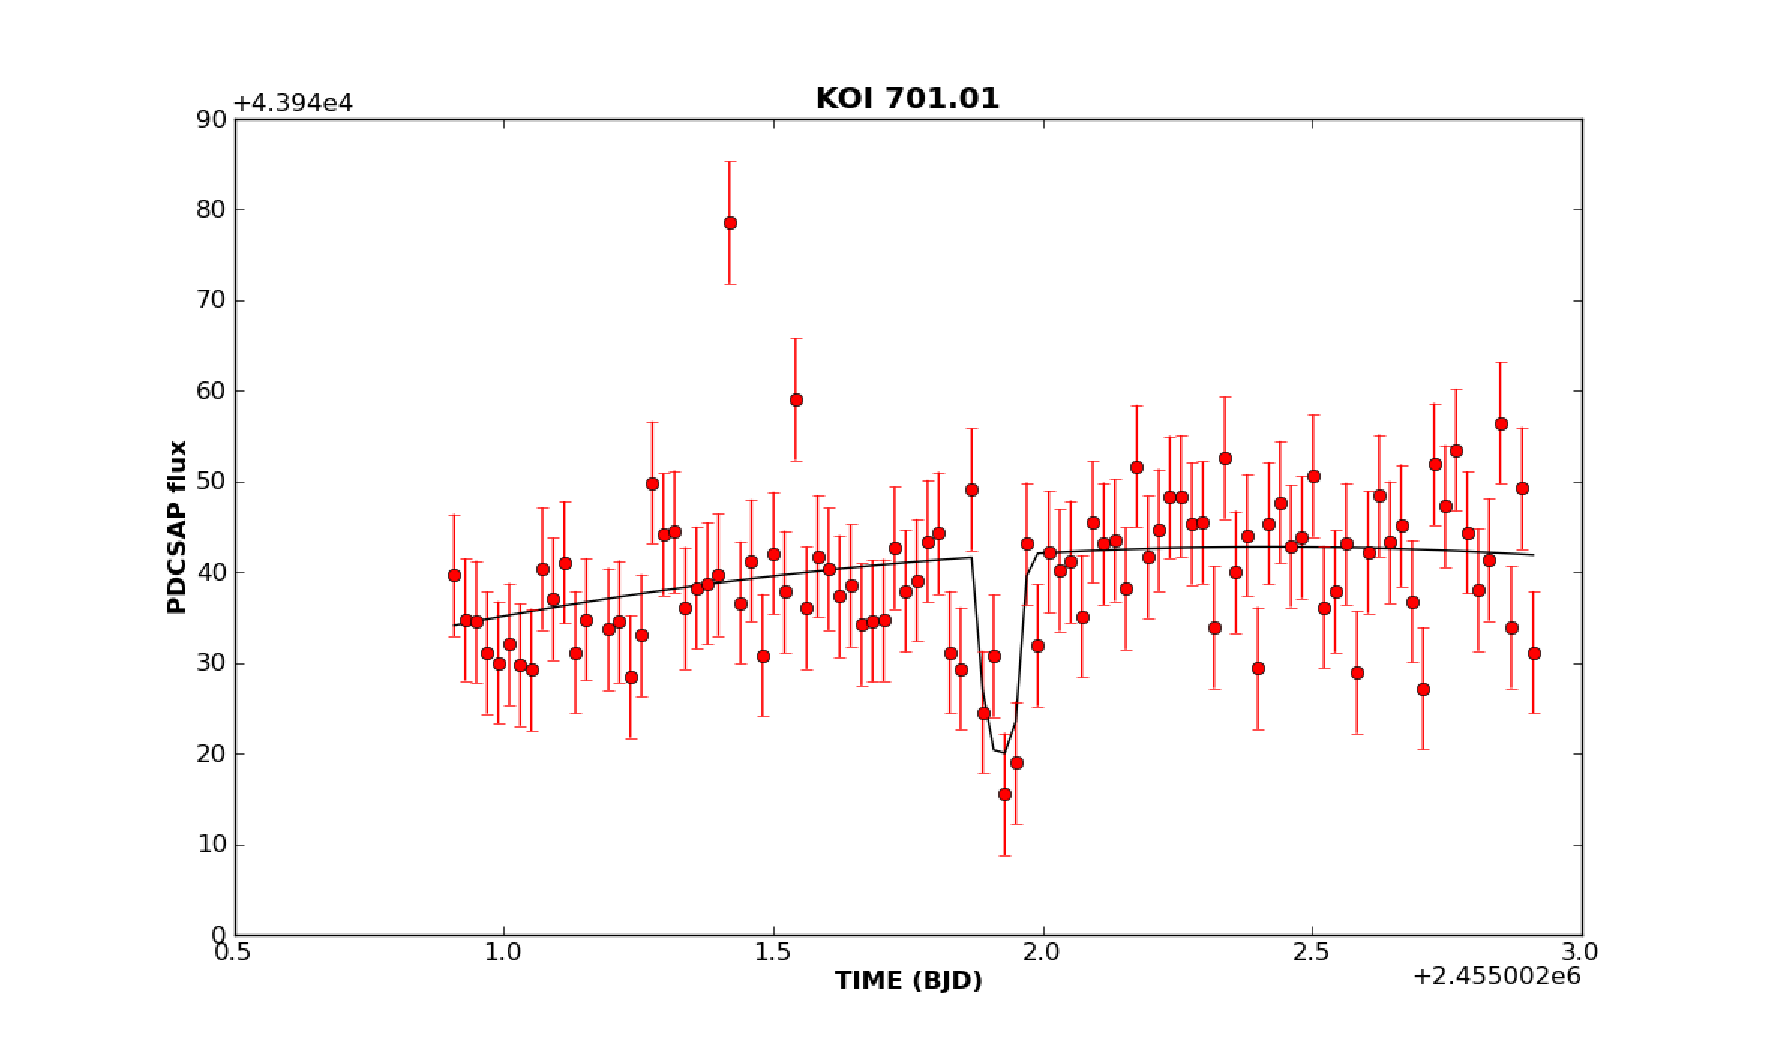
\includegraphics[width=\textwidth]{figures/701.01.eps}
  \end{minipage}\hfill
  \begin{minipage}[c]{0.4\textwidth}
    \caption{An example of our local detrending algorithm, applied to
      the first transit of KOI 701.01.  The data and model (solid
      line) are in {\tt PDCSAP} flux units.  The solid curve is
      generated by first dividing the data by the transit model,
      applying a low--order spline to the normalized data, and then
      taking the product of the spline and the model.}
    \label{fig-koi70101}
    \hspace*{\fill}  
    \hrule
  \end{minipage}
\end{figure*}

To examine how our knowledge of system parameters evolves as a
function of number of transits, we have fit {\it all} the data up to
the time of each transit, for all $N = 43$ transits in each
lightcurve.  This means that for transit $n \leq N$, we have common
model parameters $\beta_{0}^2, \tau, \zeta$ and per--transit
parameters $t_{0;i=1..n}$, for a total of $n+3$ model parameters.
This yields an ensemble of $N$ system models per lightcurve, each
incorporating one more transit than the previous one.

We used the affine--invariant MCMC sampler {\tt emcee}
\citep{2013PASP..125..306F} to sample the posterior distribution of
the model parameters.  This program uses the method of
\cite{Goodman-Weare} to achieve high sampling performance independent
of the aspect ratio of the posterior distribution, meaning covariances
between parameters are less important to the efficacy of the MCMC
sampling.  This provided a set of MCMC chains that we examine to
determine our constraints on the fitted parameters.  We used the
Gelman--Rubin $\hat{\rm R}$--static \citep{Gelman92} to assure that
each chain sufficiently samples model space, and required effective
chain lengths larger than $10^4$ to ensure sufficient mixing in the
MCMC sample \cite[e.g.][]{2004PhRvD..69j3501T}.  Our trial runs using
KOI 701.01 indicated that our chains typically have autocorrelation
lengths of $\sim 100$, requiring a total number of steps per chain of
$10^6$.  We used burn--in times having 10\% the requested number of
steps, which are then discarded before the final chain commences.

For each transit, we evaluated the joint and marginalized
distributions of fitted parameters $\zeta$ and $\tau$.
Figure~\ref{fig-joint} demonstrates how the joint distribution evolves
from fitting 1 transit (dashed contours, which represent 68.3\%,
95.5\%, and 99.7\% confidence limits), to fitting 33 transits (solid
contours, at the same confidence limits), for KOI 701.01.  We then
marginalized over all other parameters, to examine the per--parameter
confidence limits.  Figure~\ref{fig-marg} demonstrates how our
marginalized constraints on $\zeta$ (left panel) and $\tau$ (right
panel) evolved as a function of the number of transits used in the fit
for 701.01.  The solid line provides the maximum of the posterior
distribution, and the dashed line indicates its median.  The shaded
area encloses 68.3\% of the distribution.  In this manner, we find
value of $\tau = 0.056_{0.003}^{0.002}$, which is directly fitted for.
This may be contrasted to a value $\tau = 0.049 \pm 0.003 $ derived
from reported \cite{2013arXiv1304.7387B} parameters, using 171
transits.  For completeness, we note our confidence limits on $\zeta =
.01767_{0.00011}^{0.00048}$ vs \cite{2013arXiv1304.7387B} $\zeta =
0.0188 \pm 0.0003$.


\begin{figure*}[t] 
  \begin{minipage}[c]{0.47\textwidth}
    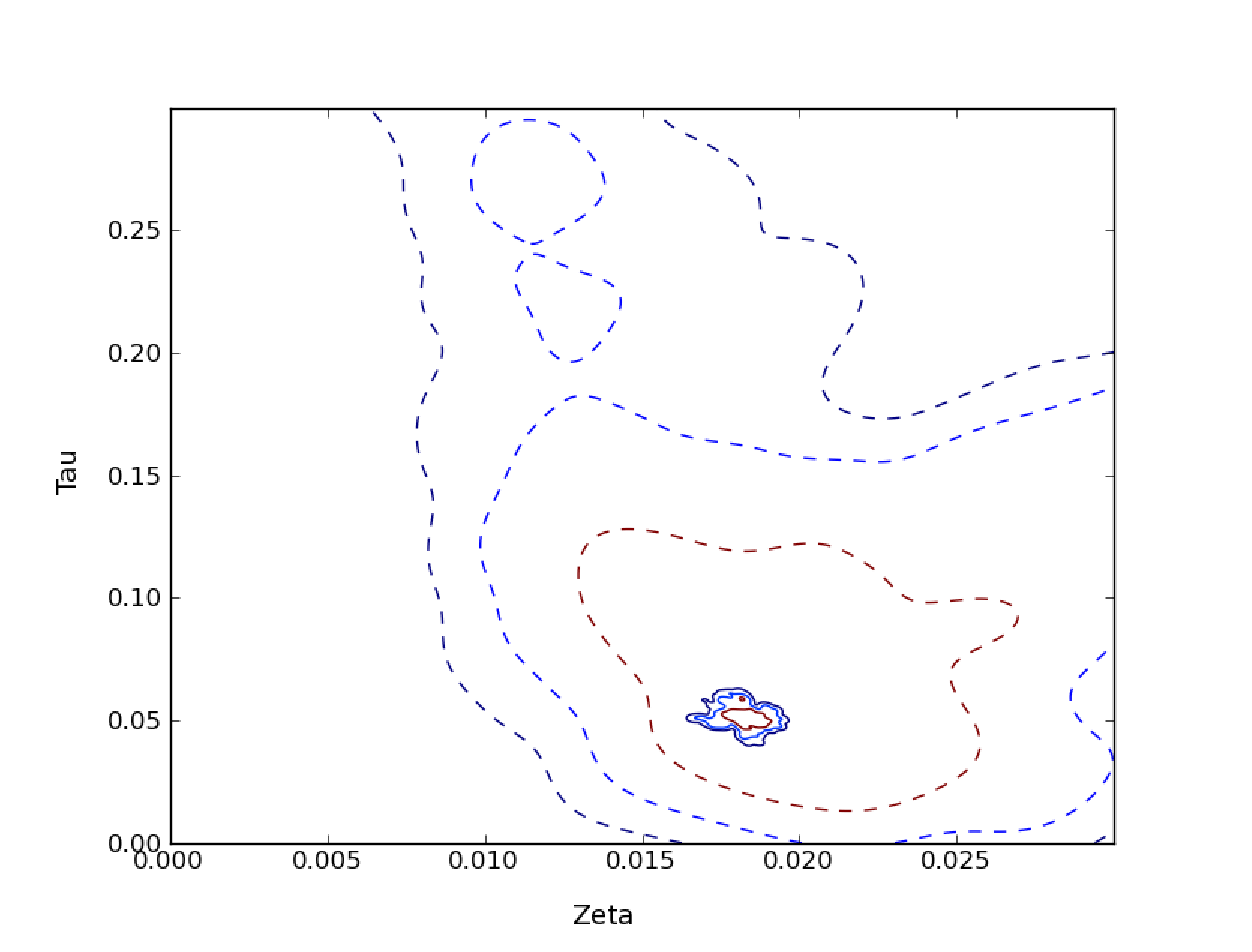
\includegraphics[width=\textwidth]{figures/joint.eps}
  \end{minipage}\hfill
  \begin{minipage}[c]{0.5\textwidth}
    \caption{The joint distribution of $\zeta$ vs. $\tau$ for KOI
      701.01.  The {\it dashed} lines show the distribution when
      fitting 1 transit, with contours at the 68.3\%, 95.5\%, and
      99.7\% confidence limits.  The {\it solid} lines show the
      distribution when fitting $N$ transits simultaneously.}
    \label{fig-joint}
    \hspace*{\fill}  
    \hrule
  \end{minipage}
\end{figure*}


\begin{figure*}[t] 
\begin{center} 
\mbox{
\subfigure{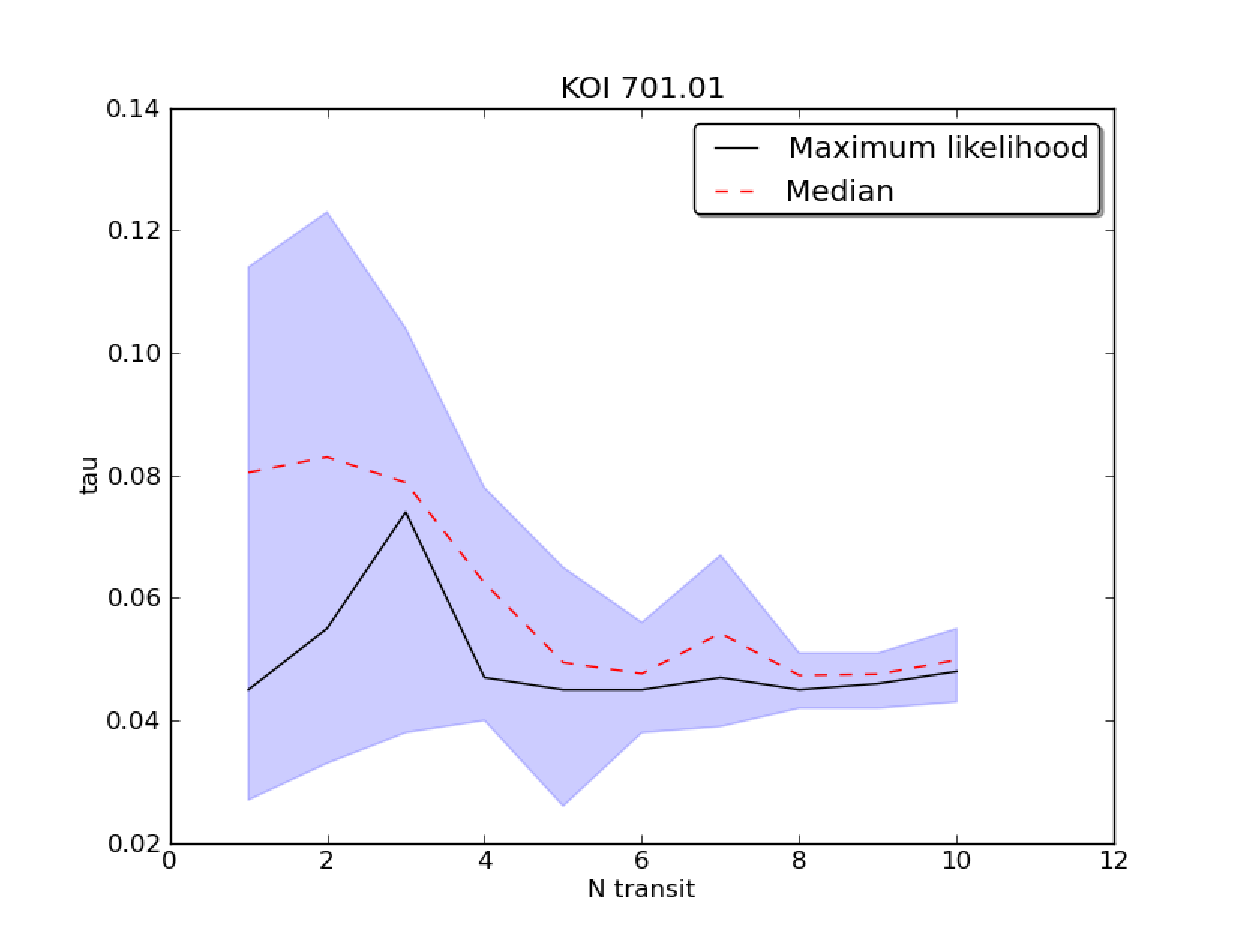
\includegraphics[width=0.47\textwidth]{figures/tau.eps}}
\quad
\subfigure{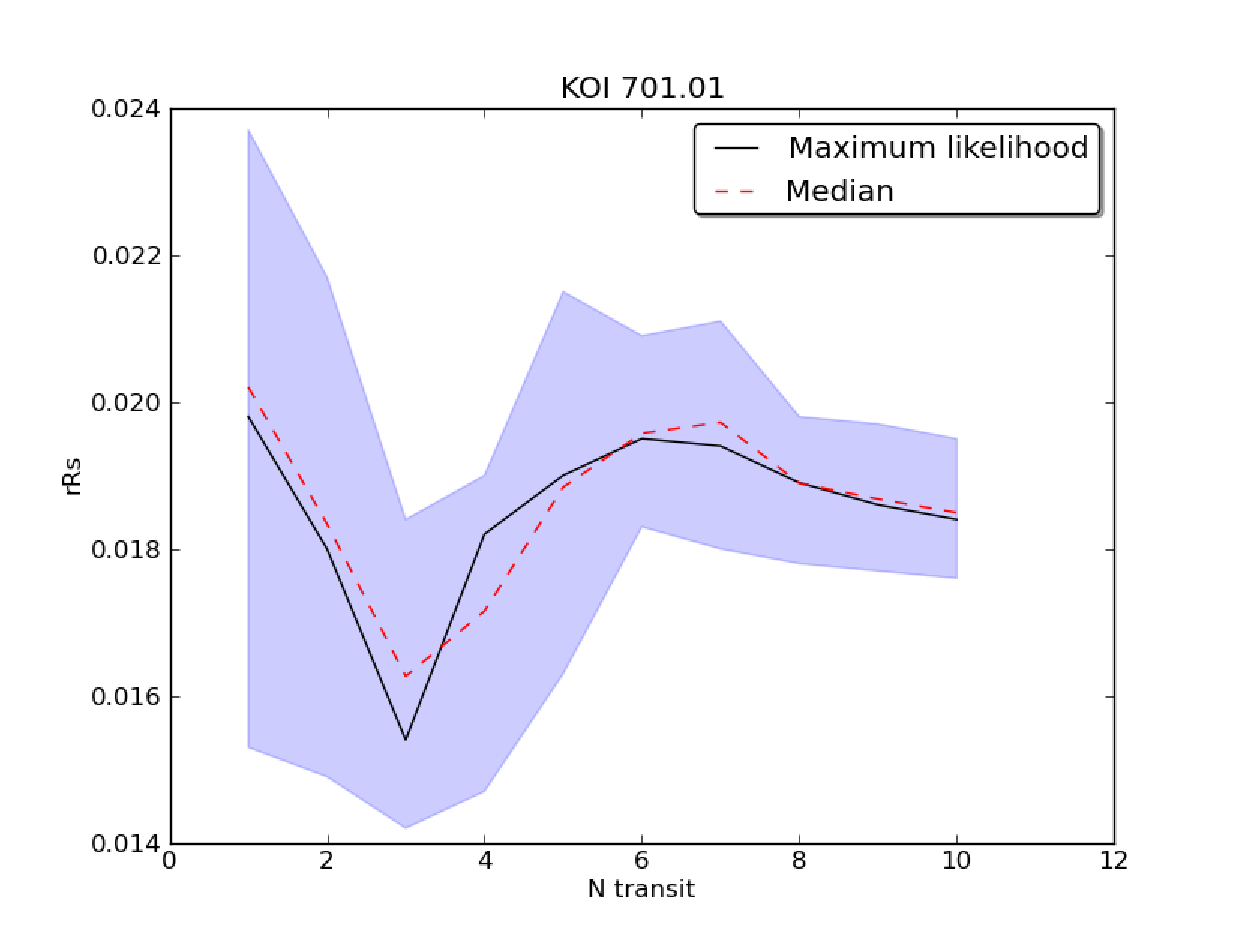
\includegraphics[width=0.47\textwidth]{figures/rRs.eps}}
}
\caption{The marginalized distributions of $\tau$ (left panel) and
  $\zeta$ (right panel) as a function of the number of transits being
  used, for KOI 701.01.  For each transit $n \leq N$ we use {\it all}
  data up to and including transit $n$ to constrain $\zeta$ and $\tau$
  (along with $\beta_0^2$ and times of transit $t_{0;i=1...n}$).  The
  {\it solid} line represents the maximum of the posterior
  distribution, while the {\it dashed} line indicates its median.  The
  shaded area contains 68.3\% of the posterior samples.}
\hspace*{\fill}  
\hrule
\label{fig-marg} 
\end{center} 
\end{figure*}

To examine our constraints on the system period, we used the
$t_{0;1..n}$ posterior distributions from the fits described above.
We used {\tt emcee} to sample the posterior space of (nuisance
parameter) $t_{0;1}$ and period $P$.  For a given trial ($t_{0;1}, P$)
pair, the likelihood was determined through:
\begin{eqnarray}
\mathcal{L}(t_{0;1}, P) & = & \prod_{i=1}^{i=n} \kappa_i(t_{0;1} + P * (i-1))
\end{eqnarray}
where $\kappa_i$ is a kernel density estimate of each posterior
distribution $t_{0;i}$, which is evaluated at the predicted time of
transit $t_0 + P * (i-1)$.  By modeling the times of transit
separately in the original MCMC analysis, we open the possibility of
using a more complex ephemeris model at this stage of the analysis,
such as may be expected from transit timing variations
\citep{2005MNRAS.359..567A,2005Sci...307.1288H}.  The results of this
analysis for KOI 701.01 are presented in Figure~\ref{fig-period}.

For the derived period, we find $P = X_{X}^{X}$.  This may be
constrasted to $P = 5.714932 \pm 0.000009$ days
from \cite{2013arXiv1304.7387B}.

The differences
in $e_{min}$ are more substantial, as our value (using the 




\begin{figure*}[t] 
  \begin{minipage}[c]{0.47\textwidth}
    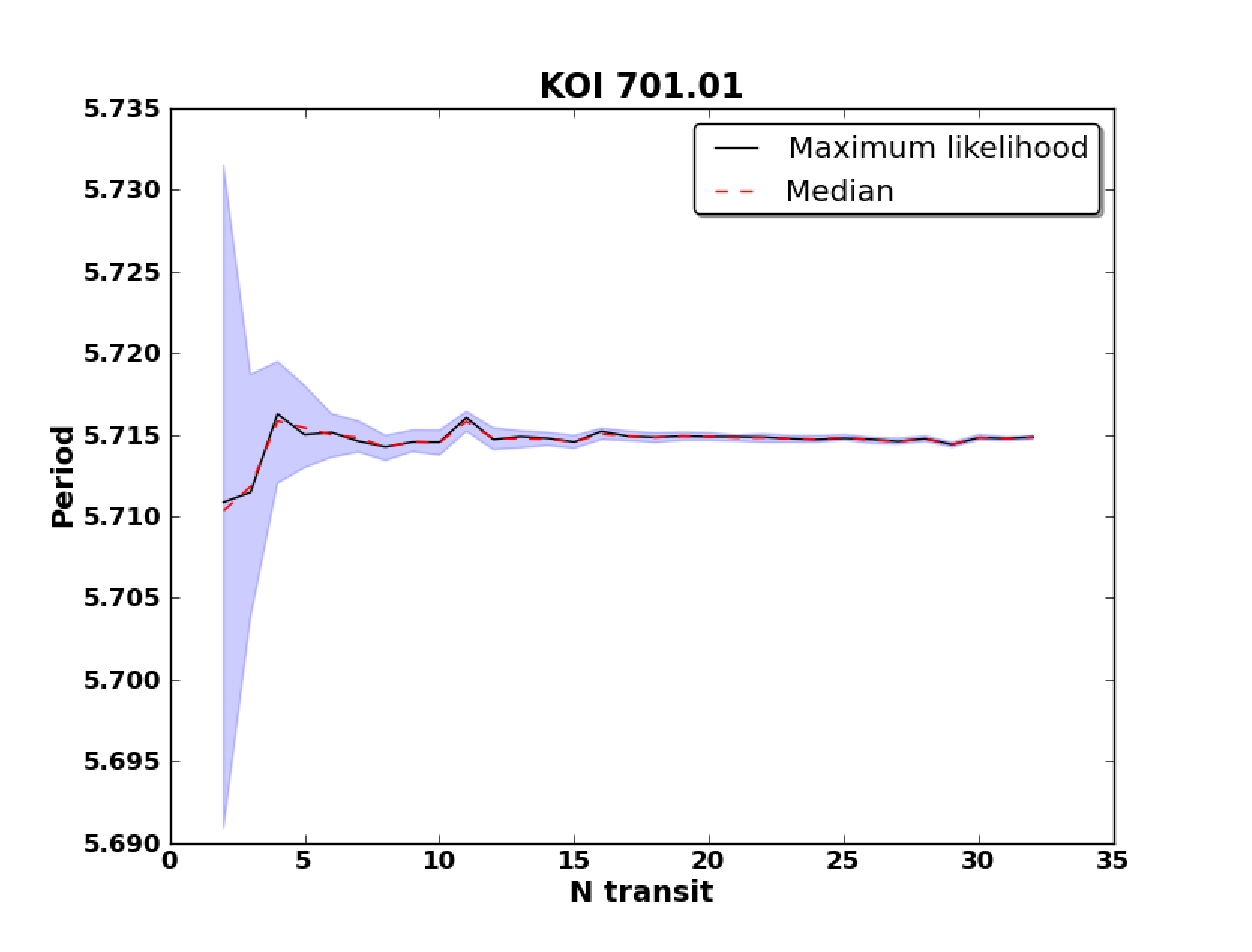
\includegraphics[width=\textwidth]{figures/period.eps}
  \end{minipage}\hfill
  \begin{minipage}[c]{0.5\textwidth}
    \caption{The evolution of the posterior distribution on orbital
      period $P$ (y--axis) based upon the results of modeling $n$
      times--of--transit (x--axis) separately.  The period posterior
      is generated by taking the product of the time--of--transit
      posteriors ($t_{0;i=1..n}$) evaluated at the predicted transit
      time $t_0 + P * i$, where $t_0$ is the (marginalized over) time
      of the first transit.  }
    \label{fig-period}
    \hspace*{\fill}  
    \hrule
  \end{minipage}
\end{figure*}


For our simulated data, Table~\ref{tab-taurun} lists the numbers of
transits that are needed to recover $\tau$ to 10\% as a function of
the system brightness and transit depth.

\begin{table}[t]
\begin{center}
\caption{\label{tab-taurun} Number of transits needed to recover $\tau$ to 10\%}
\begin{tabular}{c|cccc}
\hline \hline
Transit Depth (\%) & Magnitude=8 & Mag=10 & Mag=12 & Mag=14\\
\hline
5e-5 & x & x & x & x \\
1e-4 & x & x & x & x \\
5e-4 & x & x & x & x \\
1e-3 & x & x & x & x \\
5e-3 & x & x & x & x \\
1e-2 & x & x & x & x \\
\hline
\end{tabular}
\end{center}
Estimates of the number of transits needed to recover the value of
$\tau$ to 10\%, based on our simulated systems.  We determine this as
a function of transit depth, and the signal--to--noise of the
lightcurve (here, determined solely by the host star brightness).  We
combine all MCMC chains up to and including the transit listed here to
determine the multi--transit constraint on the distribution.
\hspace*{\fill} \\
\hrule
\end{table}

\medskip
{\centerline{\ub{\sc Kepler Sample Available for Analysis}}}
\smallskip

We need systems that are observed with the short cadence (ummm, maybe
not since we marginalize over $\beta_0$), are bright enough to resolve
$e_{min}$ to within 0.1, and have short period planets (less than 4
days).  From this sample, we will need to know the physical
characteristics of stellar mass and radius, and (ideally) age.

The detailed \cite{2013arXiv1304.7387B} analysis of Kepler 62--b
results in an $e_{min}$ value of $0.022 \pm 0.005$.  Contrasting this
value with distribution of publicly available data in
Figure~\ref{emin} indicates that this project {\it requires} a
complete re--analysis of relevant systems.

\medskip
{\centerline{\ub{\sc Computational Requirements}}}
\smallskip

Using KOI 701.01 as a benchmark, we find a roughly quadratic
relationship for the total {\tt emcee} computation time vs the number
of transits: $time(n) = -12.5 + 32.2 \times n + 11.9 \times n^2$
seconds (on a single 2.13 GHz core).  This relationship was
established using a fixed number of 100 burn--in and 1000 ``final''
steps for each of $2 \times n + 6$ walkers (i.e. 2 walkers for each
parameter in the model).  If we scale these chains up to $10^6$ total
steps, which should yield effective chain lengths of $\sim 10^4$, we
find a linear relationship in the computation time required to reach
$10^6$ steps: $time_{10^6}(n) = -1105 + 5943 \times n$ seconds.  For a
typical short--period system having 500 transits, this comes out to
approximately 35 CPU--days of analysis.  The {\tt emcee} code is
natively able to use multiprocessing capabilities, making this trivial
to implement on a multi--core system.  However, with {\tt XXX} systems
on our analysis path, this will require {\tt YYY} CPU--years of
computation, requiring the use of NASA's High-End Computing (HEC)
facilities.  We will also make use of the local {\tt Hyak} compute
cluster when it is available.

\medskip
{\centerline{\ub{\sc Data Interpretation}}}
\smallskip

In the following sections, we describe the theoretical component of
our research plan in more detail.  In Task A, we consider systems
consisting of one star and one planet.  In Task B, we include multiple
planet systems. In Task C, we incorporate mass loss.

\medskip
{\centerline{\ub{\sc Task A: Tides in Star--Planet Systems}}}
\smallskip

We begin with the simplest treatment, a single planet orbiting a
single star in an orbit that can be modified by tides.  We will mostly
follow the procedure described for our pilot study, but will expand
the analysis to a broader range of initial conditions as well as
include alternative tidal models.  The pilot study (25,000 simulations
of $\sim 5$ Gyr each) requires about 4 hours on a modern workstation,
and therefore many such trials are easily tractable.  Co--I Barnes is
an expert in tidal effects on exoplanets
\cite{Barnes08,Jackson08,Barnes09,Barnes12}, and will use his
existing code \texttt{eqtide} that follows the prescriptions in
\cite{Barnes12}.  The free parameters are the mass--radius
relationship for both rocky and gaseous bodies, the value of
$R_{crit}$, the $Q$s of rocky and gaseous bodies, the initial
eccentricity distribution, and the age distribution of \kepler~stars.

The choices in the pilot study were necessarily limited, and we will
explore many more options during this proposal.  While we assumed that
rocky bodies were Earth--like in their composition, other scaling laws
are possible, e.g.  \cite{Seager07,Fortney07,Lissauer11}.  We will use
these other scalings for the masses of the rocky planets, as well as
mixing the models to allow for a range of compositions.  For the
gaseous planets, we will assume different densities in the range 0.5
-- 3 g/cm$^3$, and also mixed cases where the density is chosen at
random.  The value of $R_{crit}$ is the parameter we are most
interested in, and we will examine it finely, varying it from 1 to 2.5
\rearth in 0.1~\rearth intervals.  We will consider two different
models for $Q$($R$), the tidal $Q$ as a function of planetary radius.
First we will use the same differences as in the pilot study, but we
will also consider a three--tiered model, in which intermediate mass
planets have intermediate $Q$s.  Neptune, and possible even Saturn,
have a $Q$ value of $10^4$ \citep{ZhangHamliton07,Lainey12}, and hence we
must consider this possibility, too.  This also introduces a new
radius cut--off, $R_{mid}$, which we will allow to move from 2 to
5~\rearth.  The $Q$ range for these systems will have values between
3000 and 30,000.  We will randomly choose a stellar mass in the range
0.7--1.4~\msun as we are interested in FGK stars.  {\bf A sentence on
  the age distribution}. Finally, we will keep the initial
eccentricity distribution consistent with that of more distant
exoplanets.  Ultimately we expect to run several hundred of these
suites of systems, which is easily tractable on a modern multi--core
workstation.

The examples in Figs.~\ref{fig:compareQ}--\ref{fig:emin} used one
tidal model, in which the lag angle between the tidal bulge and the
perturber is constant regardless of frequency
\citep[e.g.][]{GoldreichSoter66,Jackson08}.  Another popular model
assumes that lag angle is instead a function of frequency
\citep[e.g.][]{Hut81,Matsumura10}.  We will also employ this model
with the same ranges as described above, and relating $Q$ to the time
lag $tau$ as $Q = 1/n\tau$, where $n$ is the mean motion, e.g.
\cite{Correia12}.  In reality there is no general conversion between
the two, but this relation is in common use.  Thus, our work may also
shed light on the frustrating ambiguity in determining the most
appropriate equilibrium tidal model.

\medskip
{\centerline{\ub{\sc Task B: Multi--planet Systems}}}
\smallskip

Many of the \kepler~systems are multiple.  Its likely that many
singletons are as well, but with non--transiting companions.  Mutual
gravitational interactions between planets can maintain an
eccentricity, even in the presence of strong tidal damping
\citep{MardlingLin02,GreenbergVanLaerhoven11,Correia12}.  While this
pumping cannot explain the discrepancy in Fig.~\ref{fig:emin}, it can
still prevent some planets from reaching $e_{min} = 0$, and lead to an
incorrect determination of $R_{crit}$.  To assess this possibility, we
will perform simulations of multiplanet systems undergoing tidal
damping.

Ideally these simulations would couple an N--body integrator to the
tidal models, as the former can be very accurate.  Unfortunately the
timescales are so long that such an approach is intractable.  We
therefore must use classical secular theory in which the evolution for
Gyr can be computed in seconds.  The second order theory is
insufficient for many of the cases we consider, which will have
eccentricities up to 0.9.  Therefore, we will use higher order
theories, which have been previously developed
\citep[e.g.][]{Ford00,VerasArmitage04,LibertHenrard06}.  We may also
take advantage of the high degree of coplanarity of close--in
\kepler~systems \cite{Fabrycky12}, and ignore all terms involving
inclination.  As each of these models is computationally cheap, we can
safely use the 12th order theory of \cite{LibertHenrard} to evaluate
the evolution.  

More challenging is the choice of initial conditions.  While many
\kepler~systems are multiple, we do not yet know the underlying
distribution of orbital architectures.  A full exploration of
parameter space with arbitrary multiplicity and orbital elements would
be intractable, and would be very challenging to interpret.  We
therefore will limit our study to suites of 25,000 systems with
multiplicity that follows from the observations.  Furthermore, we will
limit the size of our planetary systems to $<0.5$ AU.  More distant
companions could certainly affect the orbits of close--in companions,
but the more distant companions may also be on inclined orbits, as
demonstrated by $\upsilon$ Andromedae c and d
\citep{McArthur10,ReffertQuirrenbach11}.  Therefore, to ease both the
computational burden, and not to diverge too far into unconstrained
parameter space, we will use these constraints.  The physical
properties of the planets will be in the same ranges as above.  Co--I
Barnes has experience with secular theory
\citep{BarnesGreenberg06a,BarnesGreenberg06b}, and hence will lead
this effort.  We will perform numerical tests of stability of initial
conditions, and will throw out systems that divergently cross strong
mean motion resonances, such 2:1, 3:1, and 3:2, that lead to system
break--up \citep[e.g.][]{Gomes05}.

Additionally, it is likely that many of the close--in systems cannot
have initial eccentricities comparable to the non--tidally--evolved
planets because they would be unstable.  In those cases, the orbits
are probably close to their primordial morphologies and experience
migration during the protoplanetary disk phase.  Recently
\cite{DawsonMurrayClay13} showed compelling evidence that high
metallicity stars are more likely to host eccentric planets.
Therefore, we will make two comparisons with the \kepler~sample: the
full set and the high metallicity set.  Although this decreases our
statistical robustness, it may yield the most appropriate comparison.

\medskip
{\centerline{\ub{\sc Task C: Atmospheric Mass Loss}}}
\smallskip

In addition to tidal evolution, close--in exoplanets can also
experience mass loss as high energy radiation can liberate hydrogen
\citep{Watson81,VidalMadjar04}.  \cite{Jackson10} showed that mass
loss and tidal evolution are coupled for the case of CoRoT--7 b and
that both positive and negative feedbacks are possible.  Mass loss is
especially important in our study as a planet could transition from a
gaseous body to a rocky body during its lifetime, leading to a
two--speed evolution.

We will employ the classic mass loss of model of \cite{Watson81} in
which XUV photons liberate hydrogen atoms in the upper atmosphere.
Mass loss can be a very complicated process
\citep{Yelle04,Lammer07,Khodachenko07,Leitzinger11,Lammer13}, and with
so many unknowns for any given planet, this simple model is most
appropriate.  The key parameter in this formulation is the efficiency
of transforming incident XUV radiation into escaping atoms,
$\epsilon$.  Most studies of hot Jupiter place $\epsilon$ in the range
0.1 -- 0.4.  We will therefore explore a range of 0.05 -- 0.5 in
increment of 0.05 and apply these to the configurations of Task A and
Task B.  For the XUV flux, we will use the empirical relationship
derived in \cite{Ribas05} for G dwarfs.  While this formulation is not
strictly valid for F and K dwarfs, analogous studies do not exist for
those spectral types, and the Ribas model is probably a close
approximation.  The Watson and Ribas models are already in
\texttt{eqtide} \citep{Barnes13}, and hence minimal code improvements
are required for this step.  This final theoretical task requires
about 2--3 times more computational resources than the other two
combined, but is still dwarfed by the \kepler~lightcurve analysis, and
can easily be completed within a few months on a workstation, or on
UW's local supercomputer.

Unfortunately the inclusion of mass loss leads to a degeneracy in our
model.  The three parameters we previously discussed, $R_{crit}$,
$Q_r$ and $Q_g$, are all related to features in Fig.~[plot of
  $\avg{e}$ as a function of radius and period, that figure I showed
  you long ago].  Mass loss complicates the picture by blurring these
boundaries.  On the other hand, it is entirely possible that we will
fail to reproduce the observed $\avg{e_{min}}$ distribution without
it.  At the conclusion of Task C, we will have about 2000 suites of
simulations with different physical parameters to compare to the
\kepler~planet candidates.  If we succeed in identifying $R_{crit}$,
then planets found in the HZ of \kepler~targets can be characterized
as gaseous or rocky (and potentially habitable), independent of
knowledge of their masses.  This is the ultimate goal of this
proposal.

\bigskip
\centerline{\bf IV. Team Qualifications and Previous NASA Support}
\addcontentsline{toc}{subsection}{IV. Team Qualifications and Previous NASA Support}
\smallskip

PI Becker is PI on NASA OSS grant NNX09AB32G, ``3.5m Transit Timing
Observations at 100\% Duty Cycle'', which observed multiple transiting
exoplanet systems for evidence of transit timing variations
\citep{2011ApJ...731..123K, 2013ApJ...764....8K, 2013ApJ...764L..17B,
  2013arXiv1304.5713K}.  Much of the software developed for that
project has been modified to operate with the \kepler data, and used in
the analyses presented here.  He has considerable expertise in using
modern software packages implemented on distributed computing
infrastructures to model multi--dimensional systems.  Relevant
examples include the work done under NASA ADP grant NNX09AC77G, ``Time
Domain Studies of the 2MASS Calibration Point Source Working
Database'', for which he is also PI
\citep{2012ApJ...748...58D,2013ApJ...764...62D}.

Co--I Barnes was a Co--I on NASA OSS grant 811073.02.07.01.15
``Simulating the Initial Planetesimal Disk'' which produced the first
N-body simulation of 1 km planetesimal accretion
\citep{Barnes09_1km}. As part of this effort, Barnes used several hundred thousand hours of CPU time at NASA HPC facilities, such as the Columbia and Plaiedes supercomputers. He has published $\sim 40$ papers on tidal theory and orbital dynamics, focusing on exoplanets
\citep[e.g.][]{BarnesQuinn01,BarnesRaymond04,BarnesGreenberg06a,Barnes11,Barnes13}. 

Co--I Agol...

\bigskip
\centerline{\bf V. Relevance to NASA Programs}
\addcontentsline{toc}{subsection}{V. Relevance to NASA Programs}
\smallskip

This project addresses directly multiple objectives that are in--scope
for the Origins of Solar Systems call for proposals, including:
\begin{itemize}

\item {\bf Observations related to the formation and evolution of
  planetary systems}: Explain.

\item {\bf Theoretical investigations related to the formation and
  evolution of planetary systems}: Explain.

\item {\bf Characterization of extra-solar planets to explain
  observations of extra-solar planets}: Explain.

\item {\bf Characterization of extra-solar planets to improve
  understanding of the origins of planetary systems}: Explain.

\end{itemize}



\bigskip
\centerline{\bf VI. Project Development Plan}
\addcontentsline{toc}{subsection}{VI. Project Development Plan}
\smallskip

PI Becker will be technical lead the project for the first 1.5 years,
which will constitute the data analysis (MCMC) portion of the project.
He will work at 50\% FTE with the graduate student to implement the
computations on the \kepler sample of data.  Co--I Barnes will serve as
technical lead for the project for the second 1.5 years, as the
project transitions from analysis of the data to interpretation and
constraints on tidal evolution theory.  Co--I Agol has significant
experience in dealing with the \kepler data, including implementing
detrending algorithms to correct for correlated noise in the \kepler
data.  He will advise as--needed throughout the project.  PI Becker
will serve as the project lead throughout.

We regard the professional development of students as an important
responsibility of {\it any} research project.  In this regard, the
graduate students funded by this proposal will have the opportunity to
attend at least one relevant conference each year, and encouraged to
give oral presentations on our work.  This will become a requirement
as the project progresses.  We expect the graduate student to become
an expert in both areas of this project, both the
computational/modeling side and the theoretical side.  This student
will receive a strong dose of both data and theory, which is a
powerful combination and one not seen often enough in the field.  We
consider this dual--aspect training a strong component of this
project.

{\bf Year 1 (2014):} This first year of the project will start with PI
Becker bringing the student up to speed in modeling transit
lightcurves, in leaning Bayesian techniques, and in implementing a
robust application of the {\tt emcee} package (or other
affine--invariant sampler, if needed).  Making the software robust to
detrending errors, missing data, and initial conditions for the
samplers is a non--trivial exercise.  Discovering and understanding
the failure modes will be a main focus of this
computationally--intensive first year.  Becker will lead this effort,
and transition the student into lead during the year.  The generation
of the MCMC chains is expected to take {\tt XXX} CPU--hours, or {\tt
YYY} calendar--hours on {\tt ZZZ}. The validation of these chains
(Gelman--Rubin $\hat{\rm R}$ and effective chain lengths) is expected
to take a comparable amount of time, as some chains are expected to
have to be re--run or extended.  The goal of this first year is to
have finalized the MCMC chains on $t_0, \beta_0^2, \tau, \zeta$ for
all transits of all KOIs.  We will make these publicly available
through a {\tt github} site specifically designed for this project.
Our modeling software will also be released via {\tt github}.

{\bf Year 2 (2015):} The second year is expected to begin with the
MCMC analyses of the periods via times of transit, and transition to
theoretical interpretation of the systems.  We will start with linear
ephemeris models for all systems to estimate periods; for those
systems where this model is insufficient, we will examine transit
timing models with more complicated ephemerides.  We anticipate that
this effort will result in the publication of 1 or more ancillary
papers on the transit timings of the systems under study, with
assistance from Agol on the interpretation of the results. During this
year, Barnes will begin working with the graduate student on the
theoretical aspects of the project. They will design and simulate the
models described in Task A and publish a preliminary estimate of
$R_{crit}$, $Q_g$, and $Q_r$. During this year we will also begin
running simulations of multiplanet systems with tidal damping.

{\bf Year 3 (2016):} During the final year, we will finish all
theoretical modeling, including the incorporation of mass loss.  We
will publish a paper on the role of multiplicity in the $e_{min}$
distribution. The graduate student will perform a final analysis of
all available \kepler~data and will compare this final data set to the
synthetic data produced by the tides+multiplicity+evaporation model.
A final paper will summarize the results of the investigation,
including final values, with error estimates, for $R_{crit}$, $Q_r$,
$Q_g$, and $\epsilon$.  We will characterize the degeneracies between
these parameters using a Bayesian framework.



\bigskip
\centerline{\bf VII. Data Sharing Plan}
\addcontentsline{toc}{subsection}{VII. Data Sharing Plan}
\smallskip

All investigators are committed to the sharing of data and software.
PI Becker has been behind real--time public alert systems for many
time--domain astronomical surveys.  This includes the MACHO survey,
the Deep Lens Survey, the SuperMACHO and ESSENCE surveys, and the
SDSS--II Supernova Survey, all of which have released their events to
the public in near--real time through web pages, Astronomer's
Telegrams, IAU circulars, and VOEvents.  He has been diligent in
releasing the software and data behind publications.  This includes
the image subtraction software {\tt hotpants}, period finding software
{\tt Supersmoother}, and spatial clustering software {\tt
  OPTICS}\footnote{http://www.astro.washington.edu/users/becker/c\_software.html}
which have been used in many subsequent publications.  He is currently
working part--time on the Large Synoptic Survey Telescope (LSST),
which is both open--source and open--data.

We will version release all software developed for this project on the
publicly available open--source collaboration website
http://github.com ({\tt github} hereafter).  The website has become a
leading collaboration platform; it enables distributed users to
download code and contribute back to the project.  All code we develop
for this project will be made available under the terms of the open
source BSD
license\footnote{http://www.opensource.org/licenses/bsd-license.php}
whenever possible.  We will make a new {\tt github} account for this
project that we will use to stage code and data releases, as described
in the project development plan.  Analysis packages used in our
publications will be released as {\tt
  iPython}\footnote{http://ipython.org} notebooks to help establish
reproducible research standards in the field.


